\subsection{State of the art}
To gather knowledge about the process of developing a gaming device using visual computing, the first logical step is to research the "State of the Art", I.e. what has already been successfully done, and how it has been done.

As the problem statement of this report revolves around using a webcam to control a game, it is logic to look at the most dominant solutions on the market, i.e. the Microsoft Xbox 360 Kinect, the PlayStation Move and the Nintendo Wii which will be described the following sections.

The purpose of this research is to gain an understanding of how the team behind the Kinect approached the problem of creating visual computing software, suitable for games, and what they did to solve it, in order to learn from their mistakes and, more importantly, their solutions.

\subsubsection{Development of the Kinect}
The Microsoft Xbox 360 Kinect is one of the most successful applications of computer-visual interaction made available to regular consumers of recent years, as proved by the sheer number of sold units during the first 60 days with over 8 million, making it the fastest-selling consumer-electronics device in history \parencite{Knies}.

As the Kinect is probably the most well-known visual computing device for gaming, and it is the device most closely resembling a possible product described by the problem statement, it seems logical to start by researching this.

\subsubsection*{Development:}
At the onset of development, the Xbox development team were using an algorithm that tracked a user's body movement, and used this string of information to 'predict' the movement. Not only were this method a bit unreliable, it simply couldn't keep up, at times, it was also prone to 'overloading' \parencite{Knies}, even if the algorithm could keep up with the speed of the movement, the tracking would become increasingly more inaccurate over time, and eventually crash, requiring a reset, thus making it unusable for extended game play.

\subsubsection*{Changing the approach:}
The team realized, that they had to change their approach, in order for the application to be suited for video gaming. They figured that as the algorithm crumbled due to it trying to interpret movement from a sequence and therefore trying to predict movement, rather than record it, they needed to change their approach to calculating the movement. \textit{“We couldn’t rely exclusively on context, your history, or your motion in the past. "We realized that we had to look at a single image at a time (...) We had to just look at an image and decide what your body pose was. We knew that this was, in theory, possible, because a person can do this. If you look at a photo, you can draw the position of the joints.”} - Jamie Shotton, 2011.

Instead of trying to predict something as unpredictable as human movement during games, the team figured that the application needed to interpret movement from every frame of a video stream instead - i.e. they needed an algorithm capable of reading a body's position in space from an image, converting said position into data of movement.

Research in this specific field already existed in the computer-vision literature, which made the approach seem promising.

\begin{figure}[!htbp] 
\centering
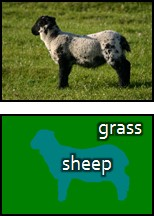
\includegraphics[scale=1]{Sheep1} 
\caption{Sheep-and-grass example.}
\label{fig:Sheep}
\end{figure}
\bigskip

The initial algorithm attempted to match the entire body at once, comparing the image with an extensive database of possible body poses - in essence, the algorithm recorded the body's pose, compared them with the entire library, until it found the best match.

To some extend, the method was functional, but it wasn't going to be efficient enough for the needs of a gaming hardware - As the algorithm checked the entire body at once, it meant that the library had to represent every possible combination of poses, meaning that the library would grow exponentially, causing it to be way too extensive. \parencite{Knies}
The team looked at the existing literature for answers, and found a way to solve the issue:

They had to break up the body into multiple different focus points - i.e. instead of labelling the entire body, they had to identify and label each joint separately.

The way they did this, was to use the "sheep-and-grass" example:
Using an image of a sheep on a grass field, the process isolates the sheep from the grass, automatically labelling the two as sheep and grass, respectively  (fig. \ref{fig:Sheep}).
\bigskip

This principle was used for the Kinect, to label and color parts of a body. Once completed and combined with the gray-scale image from the camera, it was possible to locate each joint of the body, as the colored parts are defined as being near a joint. By combining the color code of a joint, and the depth information from the gray-scale image, it was possible to estimate the 3D XYZ coordinates of the joint.

\subsubsection*{The Kinect comes to life}
With the object-recognition approach showing promise, the Xbox team started considering how to implement the algorithm on the Xbox 360 hardware, which, at the time, was already three years old. The team needed to figure out a way to implement the tracking algorithm into the existing hardware, taking the ever more demanding games into account.

To solve this, the team used machine learning, and to do this, they needed data.	
\bigskip

\textit{“Mat would feed that motion-capture data into a computer-graphics tool that generated depth images so we’d have something to test on where we knew the right answer. We had a ground-truth answer associated with each image.”} - Fritzgibbon, 2011.
\bigskip

Instead of taking images of real-life people and labelling by hand - a method which is both extremely inefficient and expensive - the team decided to synthesize images, by using computer graphics. After some initial issues with speed or reliability, the team figured out a way to generate the synthesized depth images, which enabled the team to generate millions of images, expanding the training library greatly.

The team then needed to tweak the algorithm to gain greater accuracy, expanding the training library as they went. One problem became apparent, however: it took a very long time to 'train' the program, making the application slow and cumbersome. Using an algorithm dubbed Exemplar ,an algorithm used for object removal and labeling in digital images, \parencite{Cheng2005}, they solved this issue, enabling the application to work fast and accurately enough to run on every single frame of the data-stream of the Kinect depth camera.

Once this was up and running, the team further tweaked the algorithm, enabling them to turn the application to provide a full skeleton, instead of joints, to provide temporal coherence.

By the time the algorithm had been completed, it was capable of processing 30 frames per second, using only 10\% of the Xbox's processing power - thus making it usable for gaming, as less processing power used by controllers (i.e. the Kinect), means more processing power for the actual games.

\subsubsection*{Summary:}
Instead of tracking 'nameless' objects in a stream of images, a reasonable alternative is to record, divide, and label each section of an image - i.e. each joint of a body, keeping track of each part of a body individually, instead of trying to record the body as a whole. This saves processing power, and increases reliability and accuracy.